%!TeX root =  ../../thesis.tex

\subsection{Arduino}
Arduino je open source platforma původem z Itálie, v základu se jedná o mikrokontrolér se zabudovaným programátorem, tudíž není potřeba externí programátor čipů, což usnadňuje prototypování různých zařízení. Adrudio mikrokontroléry se dělají od velmi malých (Arduino Nano 33 BLE) po velké (Arduino Mega), které je určeno pro velké projekty, kde je potřeba prostor komplexní instrukce nebo propojení s větším množinovým komponentů, nejpopulárnější je však “Arduino Uno”, které je takový “zlatý střed”.

\begin{figure}[h!]
	\centering
	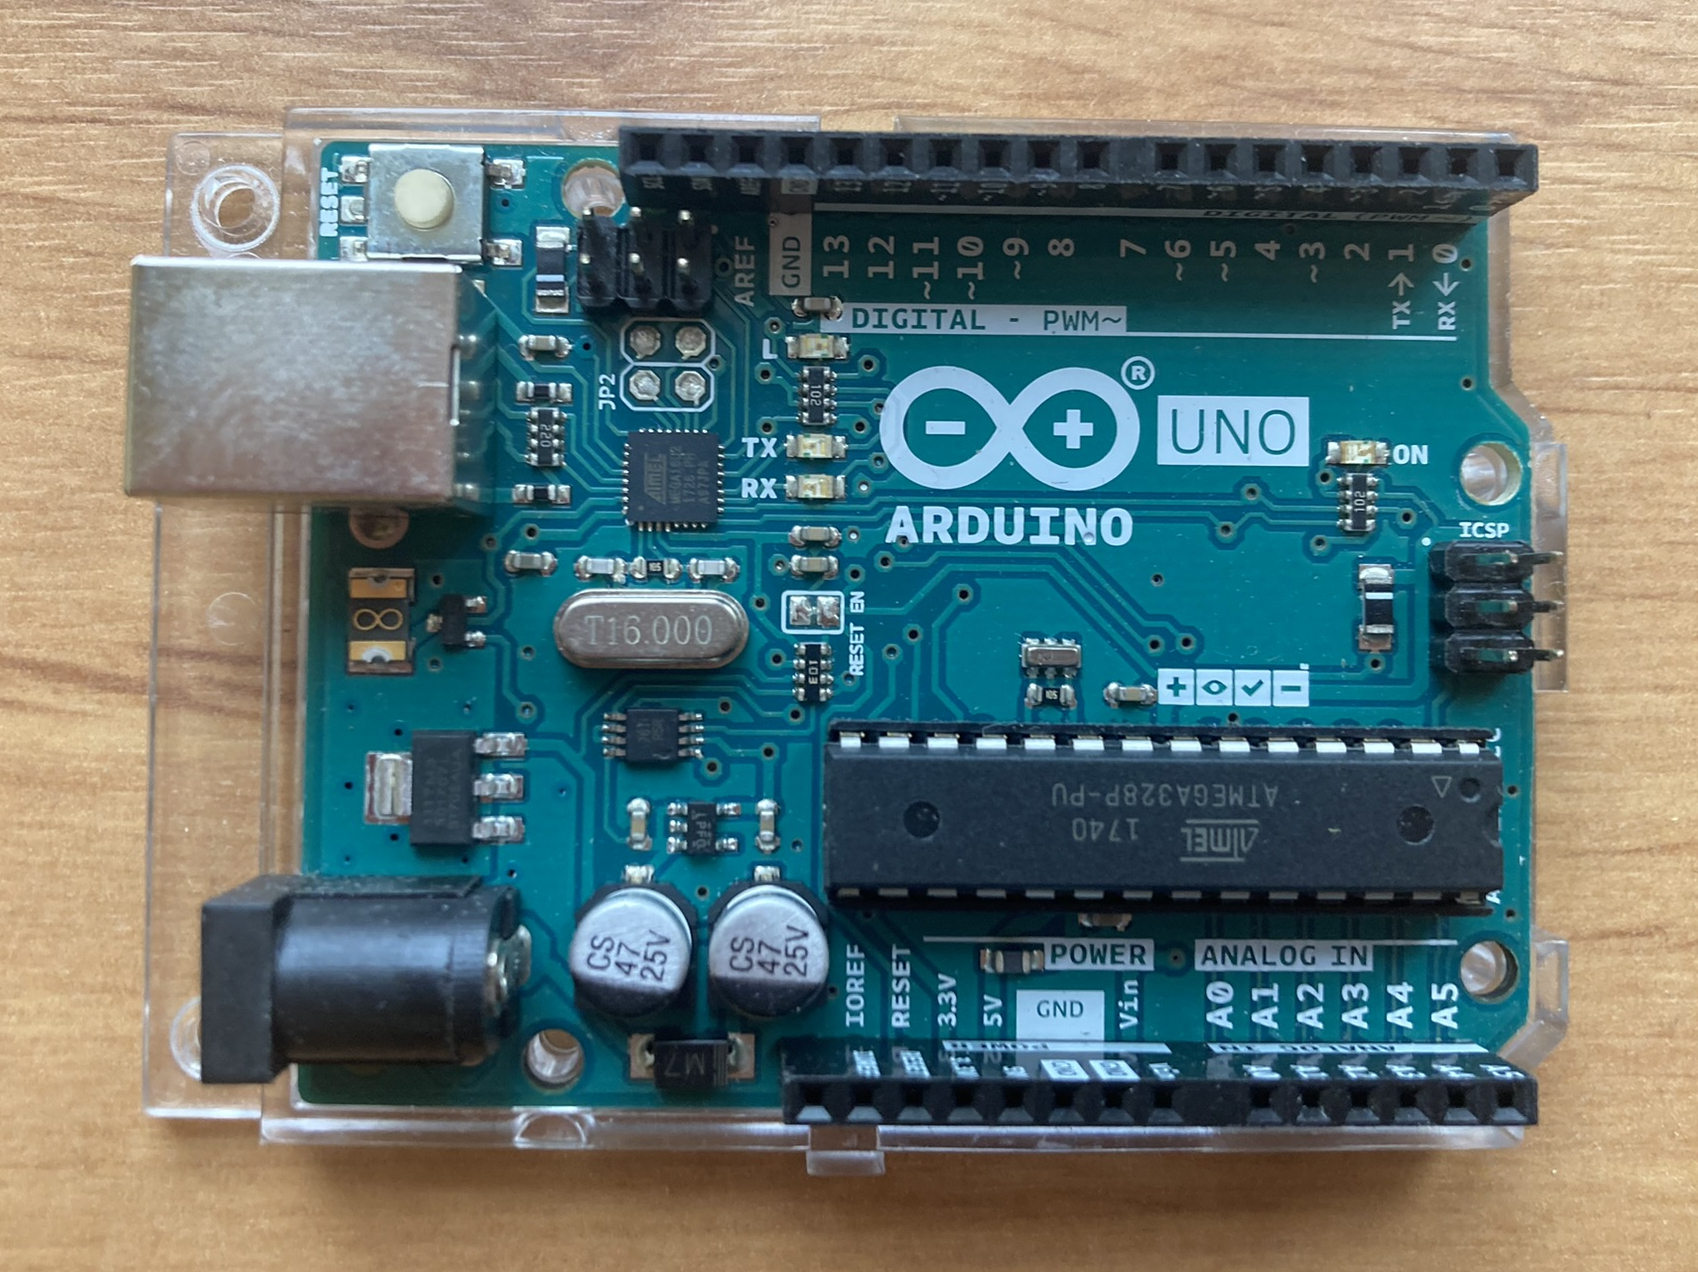
\includegraphics[width=0.9\textwidth]{pictures/arduino.jpeg}
    	\caption{Arduino Uno}
   	\label{fig:arduinoUno}
\end{figure}	

Na obrázku \ref{fig:arduinoUno} vidíme Arduino Uno, z potisku vidíme, že má digitální piny, které umí být i digitální. Jedná se o opravdu jednoduchý mikrokontrolér, avšak je velmi užitečný ve svojí univerzálnosti a nebýt potřeby pro velké množství IO tak bych použil pro vytvoření testeru právě Arduino Uno. Arduino Uno na obrázku má mikroprocesor ATmega 328P, který není sice miniaturní, ale dodává Arduinu potřebný výpočetní výkon, proto je tento model tak univerzální a dělá se i s úpravou kdy je možné využít WiFi či Bluetooth (tá má už však jiný mikroprocesor). Zajímavost na závěr, na tomto Arduinu je vidět, jak ledka, která je programovatelná, je blízko pinu číslo 13 a to pro to, že snad na většině Arduino desek je programovatelná ledka spojená s pinem 13. Což znamená, že z pinu 13 se nedá přečíst 5V signál spolehlivě, jelikož ledka a pullup rezistor snižují napětí, které je posíláno do pinu 13. Technický popis proč tomu tak je je už mimo obor a téma této bakalářské práce, proto jej zde nebudu dále rozvádět.